\documentclass[12pt]{article}
\author{Alex Ho}
\title{FYS4150 - Computational Physics \\ Project 4}
\usepackage{listings}
\usepackage{graphicx}
\usepackage{verbatim}
\usepackage{amsmath}
\usepackage{float}
\usepackage[utf8]{inputenc}
\usepackage{xcolor}
\usepackage{booktabs}
\usepackage{hyperref}
\usepackage{placeins}
\usepackage{parskip}
\setlength\parskip{\baselineskip}
\setlength\parindent{0pt}

\lstset{
language=Python,
basicstyle=\ttfamily,
otherkeywords={self},             
keywordstyle=\ttfamily\color{blue!90!black},
keywords=[2]{True,False},
keywordstyle={[2]\ttfamily\color{blue!90!black}},
emph={MyClass,__init__},          
emphstyle=\ttfamily\color{red!80!black},    
stringstyle=\color{blue!90!black},
showstringspaces=false,
commentstyle=\color{blue!90!black},
breaklines=true,
tabsize=3,
moredelim=**[is][\color{blue}]{@}{@}
}
\begin{document}
\maketitle
\begin{abstract}

\end{abstract}
\newpage
\tableofcontents
\newpage
\section{Introduction} \label{section:intro}
In fields like thermal dynamics, one will study the phenomena called a \emph{phase transition}. Not only do we study it, but we experience this phenomena on a day-by-day basis. An example of a phase transition is when water turns to steam when we boil the water. More general, a phase transition is when matter changes it's form, either from gas to liquid, or liquid to solid (and vice versa).

We will in this project use a very popular model, the Ising model, to look at the statistical properties of phase transitions analytically. We will first consider a small $2\times 2$ lattice and see how the Metropolis algorithm compares to the analytical solutions for this system. After that, we will see how this system evolves with time as we increase the lattice size. Finally, we will take a look at phase transitions near the critical temperature for very, very large lattices.

%After that, we will use the Metropolis algorithm to see how well it works with the analytical solution and see how our system evolves with time, when we increase the grid.
All relevant files can be found in this GitHub page:

\url{https://github.com/AHo94/FYS3150_Projects/tree/master/Project4}

%In fields like thermal dynamics, one will study the phenomena called phase transitions. A phase transition is when matter changes it's form. An example of a phase transition is when water turns into ice, i.e, liquid transitions into solid matter. We will in this project study a very popular model, the Ising model, to simulate phase transitions.

\section{Method} \label{section:methods}
\subsection{The Ising model}
The Ising model is a mathematical model for magnetic systems in statistical mechanics. We will in this project consider phase transitions at finite temperatures. The energy, for a specific microstate $i$, is expressed as
\begin{align}
E_i = -J \displaystyle \sum^N_{< kl >}s_ks_l - \mathcal{B}\sum^N_k s_k
\label{eq:Energy_eq}
\end{align}
With the spins $s_k$ which can take values $s_k = \pm 1$. $N$ is the total number of spins in the system and $J$ is a coupling constant, which we will assume to be $J>0$. The symbol $< kl >$ indicates that we only sum over the nearest neighbouring spin. That is, we only the spin $s_k$ with the closest spin $s_l$. $\mathcal{B}$ is an external magnetic field that is interacting with the magnetic moment between neighbouring spins. For simplicity of this project, we will set $\mathcal{B} = 0$.\\\\
We also have the magnetization (or magnetic moment) defined as
\begin{align}
\mathcal{M} = \displaystyle \sum^N_{j=1} s_j
\label{eq:Magnetization}
\end{align}
What we are interested in is the expectation values of the energy $\langle E \rangle$ and the magnetization $\langle \mathcal{M} \rangle$. In order to do that, we will need a probability distribution
\begin{align}
P_i(\beta) = \frac{e^{-\beta E_i}}{Z}
\label{eq:Probability_dist}
\end{align}
where $\beta = 1/k_bT$, the inverse temperature with $k_b$ as the Boltzmann constant. The partition function $Z$ is given as
\begin{align}
Z = \displaystyle \sum_{i=1}^M e^{-\beta E_i}
\label{eq:Partition_func}
\end{align}
which sums over all possible microstates $M$. With these, we can calculate the expectation value of an arbitrary variable $x$
\begin{align*}
\langle x \rangle = \frac{1}{Z}\sum_i x_i e^{-\beta E_i} \\
\langle x^2 \rangle = \frac{1}{Z}\sum_i x_i^2 e^{-\beta E_i}
\end{align*} 
The variance for this variable is then
\begin{align*}
\sigma_x^2 = \langle x^2 \rangle - \langle x \rangle^2
\end{align*}
We can now use these properties to calculate the heat capacity $C_v$ and susceptibility $\chi$, which are given as
\begin{align*}
C_v &= \frac{\sigma_E^2}{k_BT^2} \\
\chi &= \frac{\sigma_M^2}{k_BT}
\end{align*}


\subsection{Metropolis algorithm and computation time}
Monte Carlo methods are widely used to solve problems in different fields in science. The idea behind Monte Carlo simulation is do statistical simulations by drawing a sequence of random numbers In this project, we will use the Monte Carlo method known as the Metropolis algorithm to solve the Ising model numerically.
The algorithm is as follows: for each Monte Carlo cycle we do:
\begin{itemize}
\item \textbf{1)} We start with an arbitrary microstate for the given lattice. We use that microstate to calculate the energy $E_b$
\item \textbf{2)} Choose a random spin in the microstate and flip it (e.g, from $\uparrow$ to $\downarrow$). Now we use that state to calculate the energy $E_t$.
\item \textbf{3)} Calculate the energy difference $\Delta E = E_t - E_b$. 
\item \textbf{4)} If $\Delta E <= 0$, we accept the new spin configuration and use the energy $E_t$. What this means is that the energy has been lowered and we are in a lower state.
\item \textbf{5)} If $ \Delta E > 0$, pick a random number $r$ that is given from a uniform distributor in the range $r \in [0,1]$. Now we have to consider these two cases
\item \textbf{5a)} If $r <= e^{-\beta \Delta E}$, we accept the new spin configuration and use the energy $E_t$.
\item \textbf{5b)} If $ r > e^{-\beta \Delta E}$, we reject this new configuration and flip the chosen spin back to it's original state and use the energy $E_b$.
\item \textbf{6)} Once that is done, we use the given microstate (depending on the cases given above) to calculate the magnetic moment $M_i$.
\item \textbf{7)} Finally, we add the calculated energy and magnetic moment to $E_{sum}$ and $M_{sum}$ respectively. These will the one sample of the Monte Carlo cycle.
\end{itemize}
We repeat this process $N_{mc}$ times (with $N_{mc}$ as the number of Monte Carlo cycles) and multiple samplings which will be summed into $E_{sum}$ and $M_{sum}$. Once that is done, we get the mean energies as
\begin{align*}
\langle E \rangle = \frac{1}{N_{mc}}E_{sum} = \frac{1}{N_{mc}}\displaystyle \sum_i E_i
\end{align*}
With $E_i$ is energy sample of the $i$'th Monte Carlo cycle. Similar expressions are used for the magnetic moment and their squares.

Since we are working with probabilities, we will have to run this algorithm many, many times. Take a dice roll as an example. We know that the probability of getting the number 3 is $1/6$. If we were to throw the dice 10 times, the probability of getting 3 will most likely not be $1/6$ any more. One have to throw the die many many times to get the expected probability. The same idea is applied for Monte Carlo methods, as one has to do many samplings to get a reasonable result. This is also why Monte Carlo simulations are known to be greedy simulations.

Because of this, doing Monte Carlo simulation will take a lot of computation time. Since we have to change all the possible spins $L$, the number of floating point operations our algorithm will be roughly $L^2$. This is not including other intermediate calculations within the algorithm. When we consider $L = 2$, the computation time will be incredibly short. However, as we increase the total number of spins to $L = 20, 40, 60, 100, 140$, the computation time will increase by roughly $400, 1600, 3600, 10 000$ and $19 600$ times respectively.

Note that this is only for one Monte Carlo cycle. As mentioned earlier, we will have to do many Monte Carlo cycles to obtain a reasonable result. This will increase the computation time to roughly $N_{mc} L^2$. On top of that, we  will have to do these simulations for different temperature $T$, so the simulations will increase yet again to roughly $N_T N_{mc} L^2$, where $N_T$ is the number of temperatures we would like to have. To save time, we will have to do Parallel computation, which will explained in the next part.

\subsection{Parallel computation}
As mentioned in the previous part, there will be very long computation time once we increase or lattice grid. In order to save time, we will have to use multiple cores, that should be provided in a modern computer or laptop, to do our simulation. The idea is to let the core work in parallel with each other, that is, to split the computation work among different cores, which will speed up our process quite significantly.

We will use openMPI to do parallel computing. One has to first specify the number of cores the computer has available, and openMPI will automatically split these cores to different nodes (or ranks). Each node will run the program separately, but we can specify certain initial numbers, or intervals, for each node. One can, for example, tell each node to do the computation for different temperatures. One can also specify which interval each nodes computes. For example, node 0 can compute the Monte Carlo cycles in the range $N_{mc} \in [0,100]$, while node 1 computes in the interval $N_{cm} \in [101, 200]$. If we were to do the latter option, we will have to keep in mind that the nodes are working separately, and the computed values will therefore be unknown to each other. We will have to merge the values together to one main node (or the master node), which can be done by using the command \texttt{MPI\_Reduce}.

The computation time will decrease proportionally with the number of cores we use for the simulation. The computation time will be roughly $(N_TN_{mc}L^2)/N_{c}$, where $N_{c}$ is the number of cores used in the computation.
\subsection{Simple 2 $\times$ 2 lattice}
We will first consider a 2$\times$2 lattice, find the analytical expression for partition function $Z$ and find the corresponding expectation value of energy $E$, mean magnetization $|M|$, specific heat $C_V$ and susceptibility $\xi$ as functions of temperature $T$. We also consider periodic boundary condition for this lattice. Once we have the analytical expressions, we will compare them to the numerical values from the Metropolis algorithm.

For this system, we will assume that every spin has two directions, i.e. our states can be either be in spin up state or spin down state (shorthand notation as $\uparrow$ or $\downarrow$ respectively).

The energy of the Ising model, without an external magnetic field $\mathcal{B}$, is given by
\begin{align*}
E_i = \displaystyle -J \sum_{<kl>}^Ns_k s_l
\end{align*} 
Where $J > 0$ is a coupling constant and $N$ is the total number of spins. The symbol $<kl>$ indicates that we only sum over the neighbours only. The values $s_k = \pm 1$ depends on which state it is in. We let $s_{\downarrow} = -1$ and $s_{\uparrow} = 1$. We also have the magnetic moment is given as
\begin{align*}
M_i = \displaystyle \sum_{<k>}^N s_k
\end{align*}
Since we have a $2\times2=4$ lattice, and we have two spin directions, then the number of microstate (or configuration) is $2^4 = 16$. What this means is that our we can have 16 different energies, as well as 16 different magnetic moment, for each respective microstate. Table \ref{table:All_microstates} shows all the possible microstates.

\begin{table}
\begin{center}
	\begin{tabular}{c c c c}
	Combinations of & ($s_1, s_2, s_3, s_4$)& $s_j = \lbrace \uparrow, \downarrow \rbrace$  = $\lbrace 1, -1 \rbrace$ &\\
	\hline 
	($\uparrow , \uparrow, \uparrow, \uparrow$) & 
	($\uparrow , \uparrow, \uparrow, \downarrow$) & 
	($\uparrow , \uparrow, \downarrow, \uparrow$)  & 
	($\uparrow , \downarrow, \uparrow, \uparrow$) \\
	($\downarrow , \uparrow, \uparrow, \uparrow$)& ($\uparrow, \uparrow, \downarrow, \downarrow$) & ($\uparrow, \downarrow, \uparrow, \downarrow$) & ($\downarrow, \uparrow, \uparrow, \downarrow$) \\
	($\downarrow, \uparrow, \downarrow, \uparrow$)& ($\downarrow, \downarrow, \uparrow, \uparrow$) & ($\uparrow, \downarrow, \downarrow, \uparrow$) & ($\uparrow, \downarrow, \downarrow, \downarrow$) \\
	($\downarrow, \uparrow, \downarrow, \downarrow$) & ($\downarrow, \downarrow, \uparrow, \downarrow$) & ($\downarrow, \downarrow, \downarrow, \uparrow$) & ($\downarrow, \downarrow, \downarrow, \downarrow$) \\
	\hline
	\end{tabular}
\caption{All the microstates possible.}
\label{table:All_microstates}
\end{center}
\end{table}

Figure \ref{fig:Lattice_illustration} shows a $2\times2$ lattice. We see that the point $s_1$ has $s_2$ and $s_3$ as the closest neighbours. Since we are considering periodic boundary conditions, then $s_1$ will connect to $s_2$ and $s_3$ twice. The energy term will then give the term $2(s_1s_2 + s_2s_3)$ for the point $s_1$. It does not include $s_4$ as it is not the closest neighbour to $s_1$. 
\begin{figure}[!h]
\centering
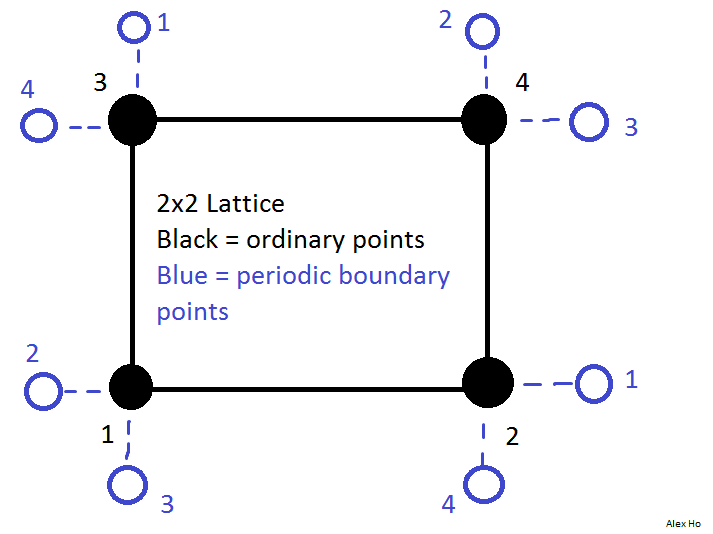
\includegraphics[width=\linewidth]{2x2_lattice_illustration.png}
\caption{An illustration of the $2\times 2$ lattice. The black points corresponds to the ordinary points $s_1, s_2, s_3, s_4$ (as point 1, 2, 3, 4 in the figure respectively). The blue points corresponds periodic boundary points.}
\label{fig:Lattice_illustration}
\end{figure}

We can then continue to add more terms using the three other points, but we need to be careful to not include the connections of the points we previously have considered, which is to prevent double counting. Doing this, the energy for each microstate $i$ will be
\begin{align}
E_i = -2J\displaystyle \sum_{s_1 = \pm1} \sum_{s_2 = \pm1} \sum_{s_3 = \pm1} \sum_{s_4 = \pm1}(s_1s_2 + s_1s_3 + s_2s_4 + s_3s_4)
\label{eq:Energy}
\end{align}
Similarly for the magnetic moment we get when we sum over all microstates 
\begin{align}
M_i = \displaystyle \sum_{s_1 = \pm1} \sum_{s_2 = \pm1} \sum_{s_3 = \pm1} \sum_{s_4 = \pm1} (s_1 + s_2 + s_3 + s_4)
\label{eq:Magnetic_moment}
\end{align}
Let us now determine both the energies and magnetic moments for all microstates. Using table \ref{table:All_microstates}, we can determine equation (\ref{eq:Energy}) and (\ref{eq:Magnetic_moment}) to their respective microstate. Table \ref{table:All_energies} and \ref{table:All_magnetic_moment} shows the energies and magnetic momenta (using the same combinations in table \ref{table:All_microstates}) respectively.

\begin{table}
\begin{center}
	\begin{tabular}{c c c c}
	$E_i =$& & &\\
	\hline
	-8J & 0 & 0 & 0\\
	0 & 8J & 0 & 0\\
	0 & 8J & 0 & 0\\
	0 & 0 & 0 & -8J\\
	\hline
	\end{tabular}
\caption{Energies for each respective microstate.}
\label{table:All_energies}
\end{center}
\end{table}

\begin{table}
\begin{center}
	\begin{tabular}{c c c c}
	$M_i = $& & & \\
	\hline
	4 & 2 & 2 & 2\\
	2 & 0 & 0 & 0\\
	0 & 0 & 0 & -2\\
	-2 & -2 & -2 & -4\\
	\hline
	\end{tabular}
\caption{Magnetic moments for each respective microstate.}
\label{table:All_magnetic_moment}
\end{center}
\end{table}

Now that we have the energies of each microstate, we can find an analytical expression for the partition function $Z$ given in \ref{eq:Partition_func}. Using the energies given in table \ref{table:All_energies}, the partition function becomes
\begin{align*}
Z = 2e^{8\beta J} + 2e^{-8\beta J} + 12 e^0 = 4\cosh(8\beta J) + 12
\end{align*}
With the partition function, we can calculate the expectation value of the energy
\begin{align*}
\langle E\rangle = \frac{1}{Z}\displaystyle \sum_i E_ie^{-\beta E_i}
\end{align*}
Summing over all states $i$, with the given energies in table \ref{table:All_energies}, we get
\begin{align*}
\langle E \rangle &= \frac{1}{Z}\left( 2(8J)e^{-8\beta J} + 2(-8J)e^{8\beta J} + 12\times0\times e^0 \right)\\
&= \frac{-32J \sinh(8\beta J)}{4\cosh(8\beta J) + 12}\\
&= \frac{-8J\sinh(8\beta J)}{\cosh(8\beta J) + 3}
\end{align*}
The expectation of the energy squared is then
\begin{align*}
\langle E^2\rangle &= \frac{1}{Z}\displaystyle \sum_i E_i^2 e^{-\beta E_i} \\
&= \frac{1}{Z} \left(2(8J)^2 e^{-8\beta J} + 2(-8J)^2 e^{8\beta J} + 12 \times (0)^2 e^0 \right) \\
&= \frac{4(8J)^2\cosh(8\beta J)}{4\cosh(8\beta J) + 12} \\
&= \frac{64J^2\cosh(8\beta J)}{\cosh(8\beta J) + 3}
\end{align*}
The standard deviation of the energy then becomes
\begin{align*}
\sigma_E^2 &= \langle E^2\rangle - \langle E \rangle^2 \\
&=\frac{64J^2\cosh(8\beta J)}{\cosh(8\beta J) + 3} - \left( \frac{-8J\sinh(8\beta J)}{\cosh(8\beta J) + 3}\right)^2 \\
&= \frac{64J^2}{\cosh(8\beta J) + 3}\left(\cosh(8\beta J) - \frac{\sinh^2(8\beta J)}{\cosh(8\beta J) + 3} \right) \\
&= \frac{64J^2}{\cosh(8\beta J) + 3}\left(\frac{\cosh^2(8\beta J) + 3\cosh(8\beta J)}{\cosh(8\beta J) + 3} - \frac{\sinh^2(8\beta J)}{\cosh(8\beta J) + 3} \right) \\
&= \frac{64J^2}{\cosh(8\beta J) + 3}\left(\frac{1 + 3\cosh(8\beta J)}{\cosh(8\beta J) + 3} \right)\\
&= \frac{64J^2}{(\cosh(8\beta J) + 3)^2}(4+\cosh(8\beta J))
\end{align*}
Dividing by $k_B T^2$ gives us the specific heat $C_V$
\begin{align}
C_V = \frac{1}{k_BT^2} \left( \langle E^2 \rangle
- \langle E \rangle^2 \right) = \frac{64J^2}{k_B T} \frac{(1+3\cosh(8\beta J))}{(\cosh(8\beta J) + 3)^2}
\label{eq:heat_capacity}
\end{align}
We can do similar calculations to obtain the mean magnetization (or the mean absolute value of the magnetic moment), which then gives us
\begin{align*}
\langle |M|\rangle &= \frac{1}{Z} \displaystyle \sum_i |M_i| e^{-\beta E_i} = \frac{2(e^{8\beta J} + 2)}{\cosh(8\beta J) + 3} \\
\langle M^2\rangle &= \frac{1}{Z}\displaystyle \sum_i M_i^2e^{-\beta E_i} = \frac{8(e^{8\beta J} + 1)}{\cosh(8\beta J) + 3}
\end{align*}
Which we can use to calculate the susceptibility $\chi$
\begin{align}
\chi = \frac{1}{k_B T} \left(\langle M^2 \rangle - \langle |M| \rangle^2\right) = \frac{8}{k_B T} \frac{(e^{8\beta J}+ \cosh(8\beta J) + \frac{3}{2}))}{(\cosh(8\beta J) + 3)^2}
\label{eq:suceptibility}
\end{align} 
Now that we have the analytical expressions, we will later compare it to the numerical values (for a given temperature) from the Metropolis algorithm.
\FloatBarrier

\subsection{Studies of phase transition}
Once we have properly tested the Ising model by using the Metropolis algorithm, we will study the behaviour of the Ising model near the critical temperature $T_C$. 

Through so-called finite size scaling relations, we can relate the behaviour of finite sized lattices with the results of an infinitely large lattice. The critical temperature then scales as
\begin{align}
T_C(L) - T_C(L=\infty) = a L^{-1/\nu}
\label{eq:crit_temp_scaling}
\end{align}
Where $a$ is a constant, and $\nu$ is defined from
\begin{align*}
\xi(T) ~ |T_C - T|^{-\nu}
\end{align*}
For our case, we will set $\nu = 1$. This is to compare the exact result of the critical temperature after Lars Onsager, which is.
\begin{align*}
\frac{kT_C}{J} = \frac{1}{\ln(1 + \sqrt{2})} \approx 2.269
\end{align*}
With $\nu = 1$. First, we will have to find what this constant $a$ is. By taking the difference of equation \ref{eq:crit_temp_scaling} for two different total spins, we have
\begin{align*}
aL_i^{-1} - aL_j^{-1} &= [T_C(L_i) - T_C(L=\infty)] - [T_C(L_j) - T_C(L = \infty)] \\
&= T_C(L_i) - T_C(L_j)\\
\implies a &= \frac{T_C(L_i) - T_C(L_j)}{L_i^{-1} - L_j^{-1}}
\end{align*}
The critical temperature for an infinitely large lattice, for a given total spin $L_i$, is then
\begin{align*}
T_C(L=_i\infty) &= T_C(L_i) - L_i^{-1}\frac{T_C(L_i) - T_C(L_j)}{L_i^{-1} - L_j^{-1}} \\
&= T_C(L_i) - \frac{T_C(L_i) - T_C(L_j)}{1 - \left(\frac{L_i}{L_j} \right)}
\end{align*}
Since we have multiple total spins, we will have to sum over all the other total spins, and then average them out. That is
\begin{align*}
T_C(L_i=\infty) = \frac{1}{N_L} \displaystyle \sum_j \left( T_C(L_i) - \frac{T_C(L_i) - T_C(L_j)}{1 - \left(\frac{L_i}{L_j} \right)} \right)
\end{align*}
Where $N_L$ is the number of all lattice sizes considered. We will for this part let the total spins be $L=40, 60, 100$ and $140$, which means that $N_L = 4$. We will also consider the temperature range $T \in [2.0, 2.3]$.

\section{Implementation} \label{section:implement}
All programming are done in C++ and data will be saved in a text file. The plotting part will be done in Python.

The main function in the C++ program is split into two parts by an if test. The if test will see if there is any arguments given in the command line. If there is none, the program will compute the simple lattice model for $L = 2$ and $L = 20$. If the there are arguments in the command line, the program will run the program for large lattices. The program will here do parallel computation, where I have decided to separate the Monte Carlo cycle interval for each node. 

There are also various of functions that is used to do all the calculations. Some of the functions have relatively similar names. One example is the \texttt{write\_file} functions. I have made two (or three, if you include the function that initializes the output file) of these functions. Both creates differently formatted output files, which is done because it will be easier to read the required data for the different tasks. 

Like my previous projects, I will plot all the data, made from the C++ program, in Python. The Python script simply reads the output file, saves the required data and then plots them.
\section{Results} \label{section:result}
\subsection*{Comparing with the analytical solution}
We will now compare the numerical values for $C_v$ and $\chi$ with their respective analytical values given in equation \ref{eq:heat_capacity} and \ref{eq:suceptibility}. For this case, we will use the temperature $T = 1.0$ in units of $kT/J$. Running this in C++, with $10^6$ Monte Carlo cycles we obtain the following output (Note that the numerical values has not been divided by the number of spins):

\begin{lstlisting}
@Number of Monte Carlo cycles = 1000000
Analytic C_v = 0.128329, Numerical C_v = 0.128445
Analytic Chi = 0.016043, Numerical Chi = 0.0162828@
\end{lstlisting}
As we can see, the values are almost identical. The numerical values may change a little bit when we run this multiple times, but still remains fairly close to the analytical values. An example of this can be found in the output below
\begin{lstlisting}
@Running multiple times, using MC_cycles = 1000000
Analytic C_v = 0.128329, Numerical C_v = 0.123027
Analytic Chi = 0.016043, Numerical Chi = 0.0156212
 
Analytic C_v = 0.128329, Numerical C_v = 0.127936
Analytic Chi = 0.016043, Numerical Chi = 0.0154724
 
Analytic C_v = 0.128329, Numerical C_v = 0.130357
Analytic Chi = 0.016043, Numerical Chi = 0.0164741
 
Analytic C_v = 0.128329, Numerical C_v = 0.125385
Analytic Chi = 0.016043, Numerical Chi = 0.0152174
 
Analytic C_v = 0.128329, Numerical C_v = 0.126915
Analytic Chi = 0.016043, Numerical Chi = 0.0156962
 
Analytic C_v = 0.128329, Numerical C_v = 0.124365
Analytic Chi = 0.016043, Numerical Chi = 0.0159204@
\end{lstlisting}
Using $10^5$ Monte Carlo cycles can also give a good numerical result, but it is not as consistent compared to $10^6$ Monte Carlo cycles. What that means is that the difference between the analytical and numerical values (for both $C_v$ and $\chi$) may be larger for a lower number of Monte Carlo cycles. The output below shows an example with $N_{mc} = 10^5$. Notice how, for example, the numerical values of $C_v$ can be as low as $0.112442$ and as high as $0.160237$.
\begin{lstlisting}
@Running multiple times, using MC_cycles = 100000
Analytic C_v = 0.128329, Numerical C_v = 0.125194
Analytic Chi = 0.016043, Numerical Chi = 0.0163315
 
Analytic C_v = 0.128329, Numerical C_v = 0.112442
Analytic Chi = 0.016043, Numerical Chi = 0.0130196
 
Analytic C_v = 0.128329, Numerical C_v = 0.123282
Analytic Chi = 0.016043, Numerical Chi = 0.0152538
 
Analytic C_v = 0.128329, Numerical C_v = 0.137304
Analytic Chi = 0.016043, Numerical Chi = 0.0180454
 
Analytic C_v = 0.128329, Numerical C_v = 0.125832
Analytic Chi = 0.016043, Numerical Chi = 0.0161317
 
Analytic C_v = 0.128329, Numerical C_v = 0.160237
Analytic Chi = 0.016043, Numerical Chi = 0.0194764@
\end{lstlisting}

\subsection*{Lattice with L = 20}
We will now increase our lattice to a $20\times 20$ lattice.  For this task, we will have a look at how the mean energy and mean magnetization (absolute value) will reach an equilibrium as a function of the number of Monte Carlo cycles. Monte Carlo cycles will represent the time for this case. This will be done for temperatures at $T=1.0$ and $T = 2.4$. We will also consider two different cases. One where all the spins in the system is randomly set and one where all spins are pointing up.
 
Let us first consider the case where the initial spin state is set at random. Figure \ref{fig:Energy_stab_log_T1} and \ref{fig:Mag_stab_log_T1} are plots of the expectation values of energy and magnetization respectively, as a function of time (the number of Monte Carlo cycles) for $T = 1.0$. The x axis is plotted in logarithmic scales to better show how the  expectation values stabilizes over time. Non-logarithmic x-axis of these plots can be found in the appendix (also found in my GitHub page). We see that both parameters stabilizes fairly quickly, even though we start in a random spin state.

\begin{figure}[H]
\centering
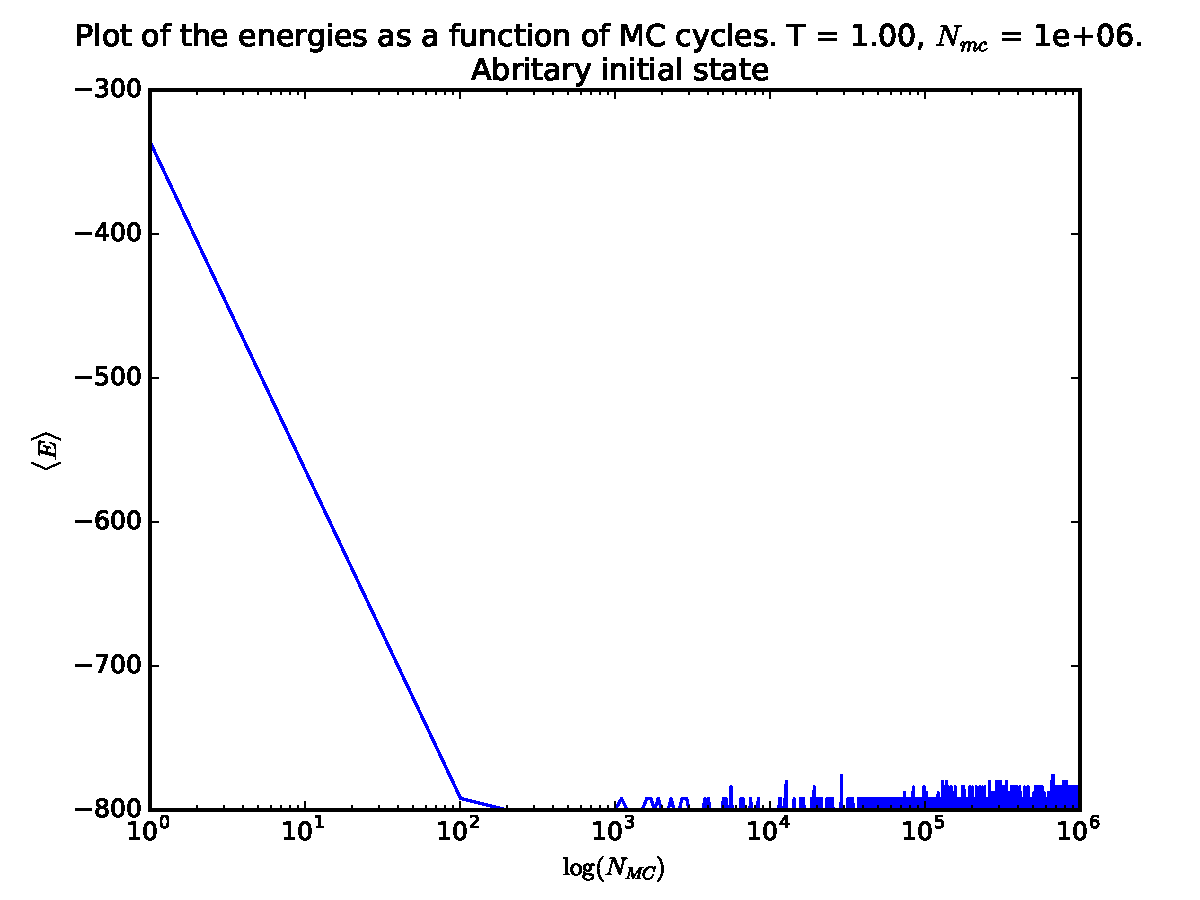
\includegraphics[width=\linewidth]{Plots/Energy_stability_logarithmic_T1.pdf}
\caption{Stability of the energy, with $T = 1.0$ as a function of time. Logarithmic x-axis.}
\label{fig:Energy_stab_log_T1}
\end{figure}
\begin{figure}[H]
\centering
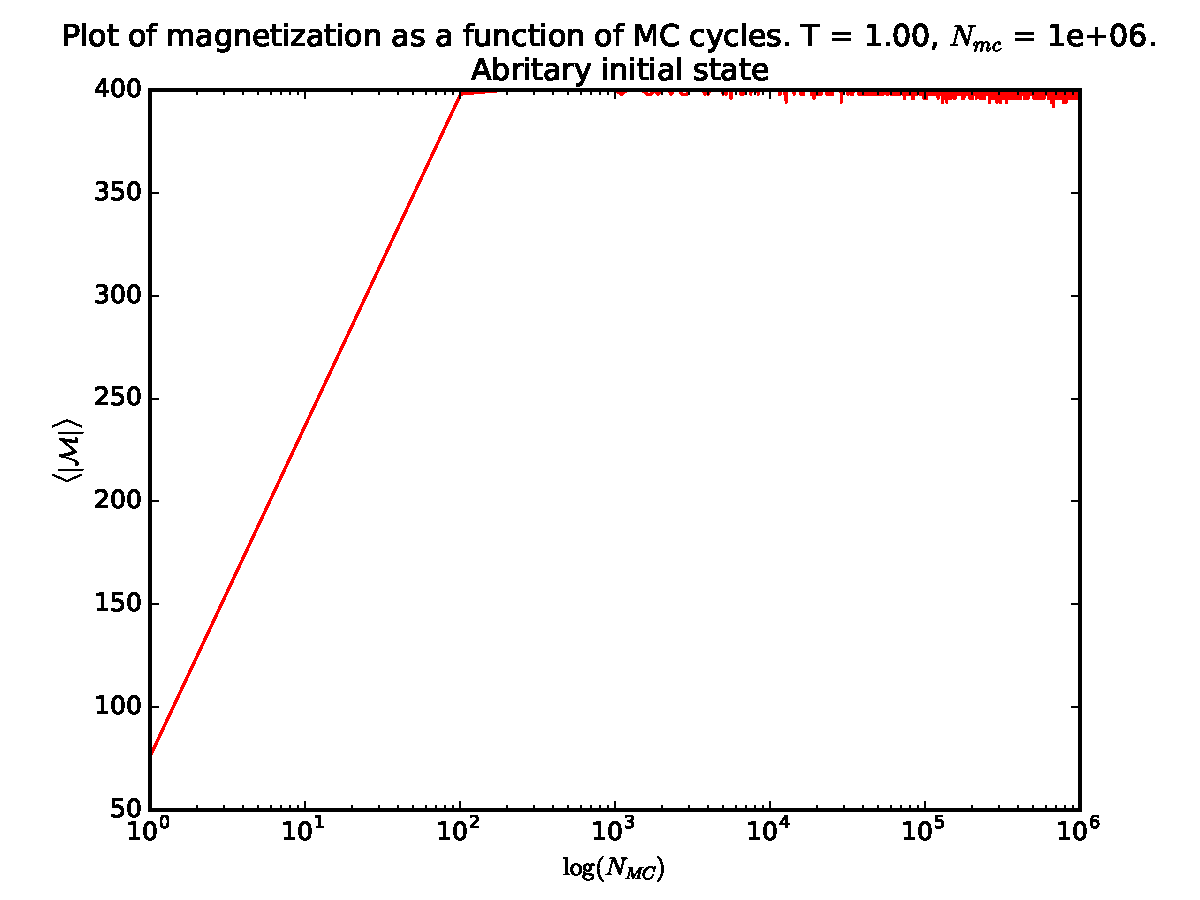
\includegraphics[width=\linewidth]{Plots/Magnetization_stability_logarithmic_T1.pdf}
\caption{Stability of the magnetization, with $T = 1.0$ as a function of time. Logarithmic x-axis.}
\label{fig:Mag_stab_log_T1}
\end{figure}

We now increase the temperature to $T = 2.4$. Figure \ref{fig:Energy_stab_log_T2} and \ref{fig:Mag_stab_log_T2} again shows how the energy and magnetization stabilizes respectively. This time, however, there are a lot more fluctuations for both parameters. This is not surprising. When we have a higher temperature, the system can reach a higher energetic state. Because of this, the spins will have the ability to change more (that is, more frequent flips) compared to the lower temperature case.

\begin{figure}[H]
\centering
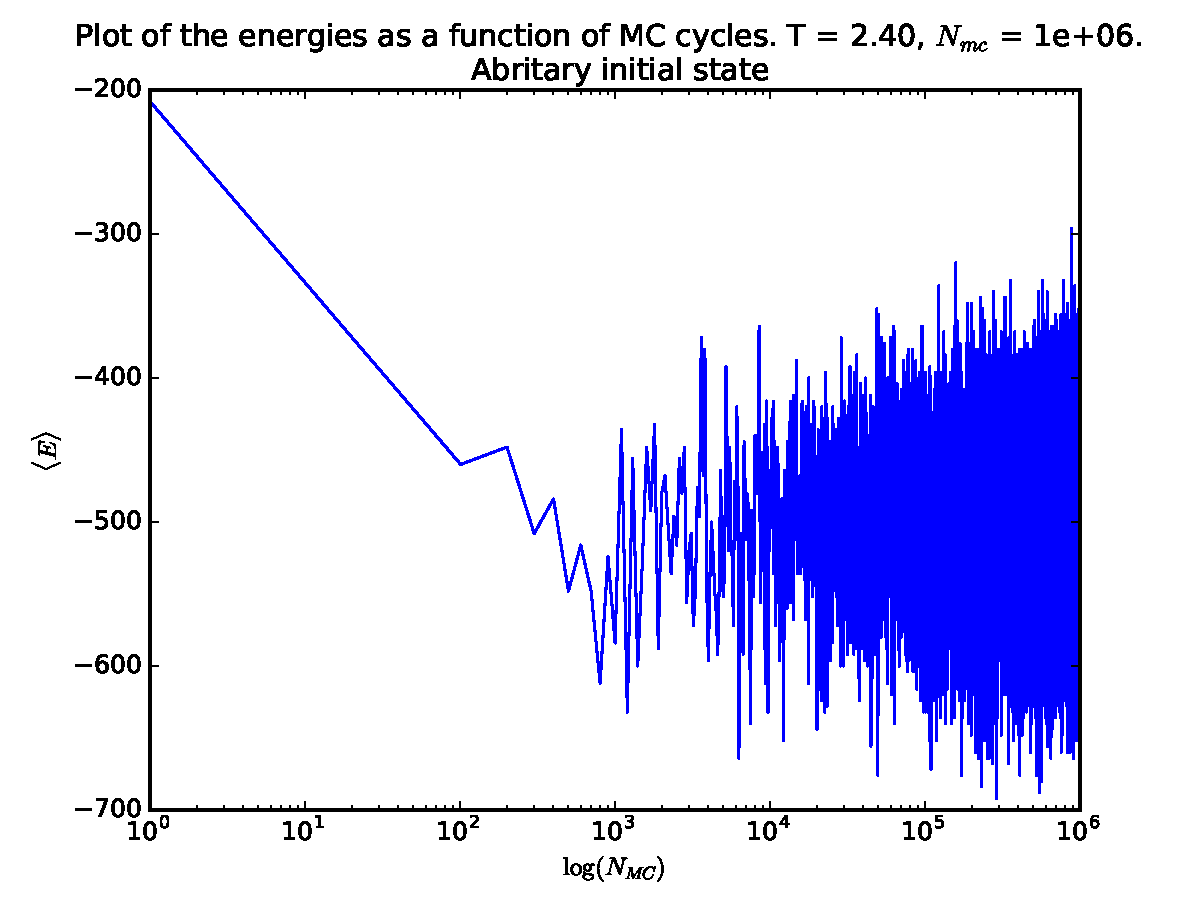
\includegraphics[width=\linewidth]{Plots/Energy_stability_logarithmic_T24.pdf}
\caption{Stability of the energy, with $T = 2.4$ as a function of time. Logarithmic x-axis.}
\label{fig:Energy_stab_log_T2}
\end{figure}
\begin{figure}[H]
\centering
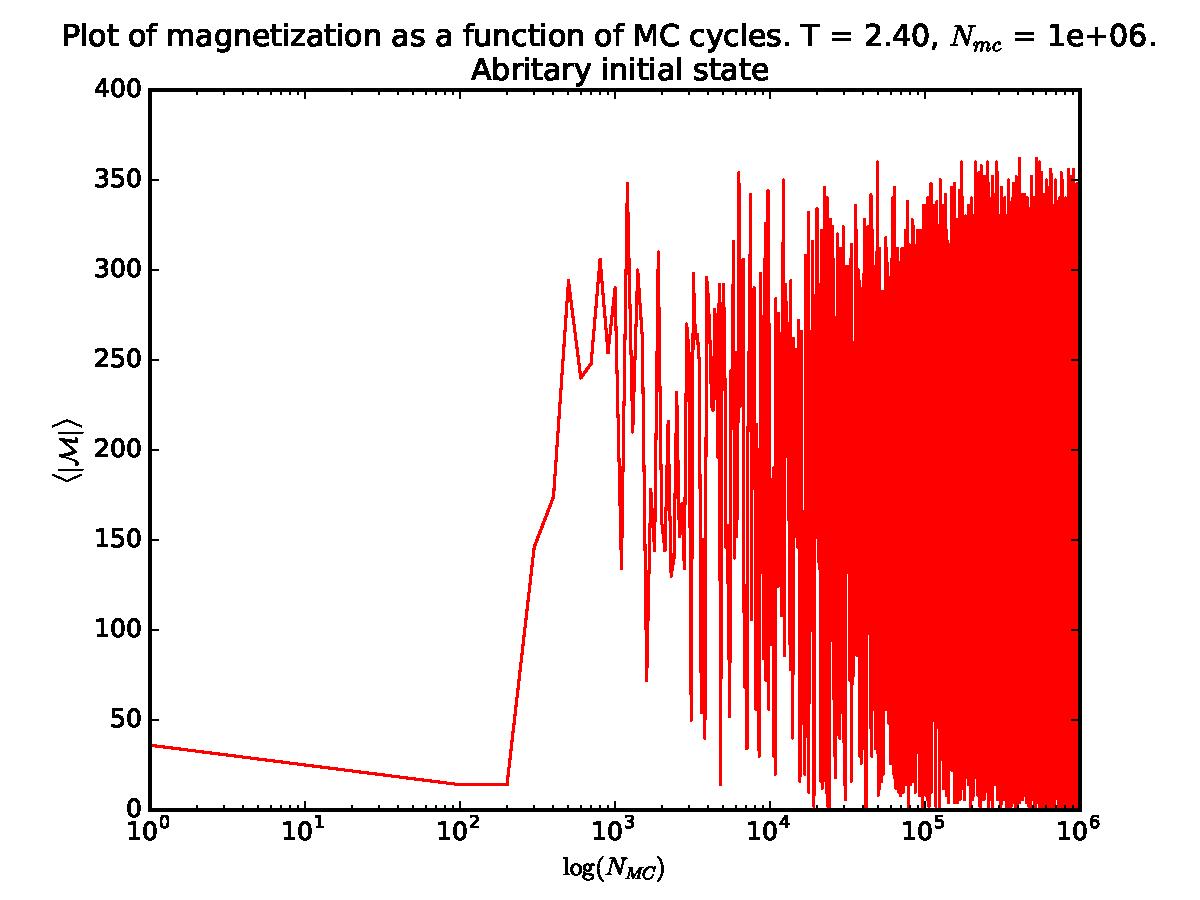
\includegraphics[width=\linewidth]{Plots/Magnetization_stability_logarithmic_T24.pdf}
\caption{Stability of the magnetization, with $T = 2.4$ as a function of time. Logarithmic x-axis.}
\label{fig:Mag_stab_log_T2}
\end{figure}


We can also have the program count how many times the a new configuration have been accepted. In figure \ref{fig:Accepted_configs_wrt_temp}, we see that we accept a lot more configurations as the temperature increases. The y-axis for this plot is in logarithmic scale. Note that I have only plotted two temperature points in the plot, so the number of accepted configurations may or may not increase linearly with temperature. This result agrees with the stability plots for $T=2.4$ that we saw earlier. 

Figure \ref{fig:Accepted_configs_wrt_MC_cycles} shows how the number of accepted configurations increases over time. The y-axis is once again logarithmic. Once again, we see that the number of accepted configurations is higher for a higher temperature. Notice how we accept a lot more configuration changes at early times, and as time passes, we accept less. This indicates that the system is going towards equilibrium. 

\begin{figure}[H]
\centering
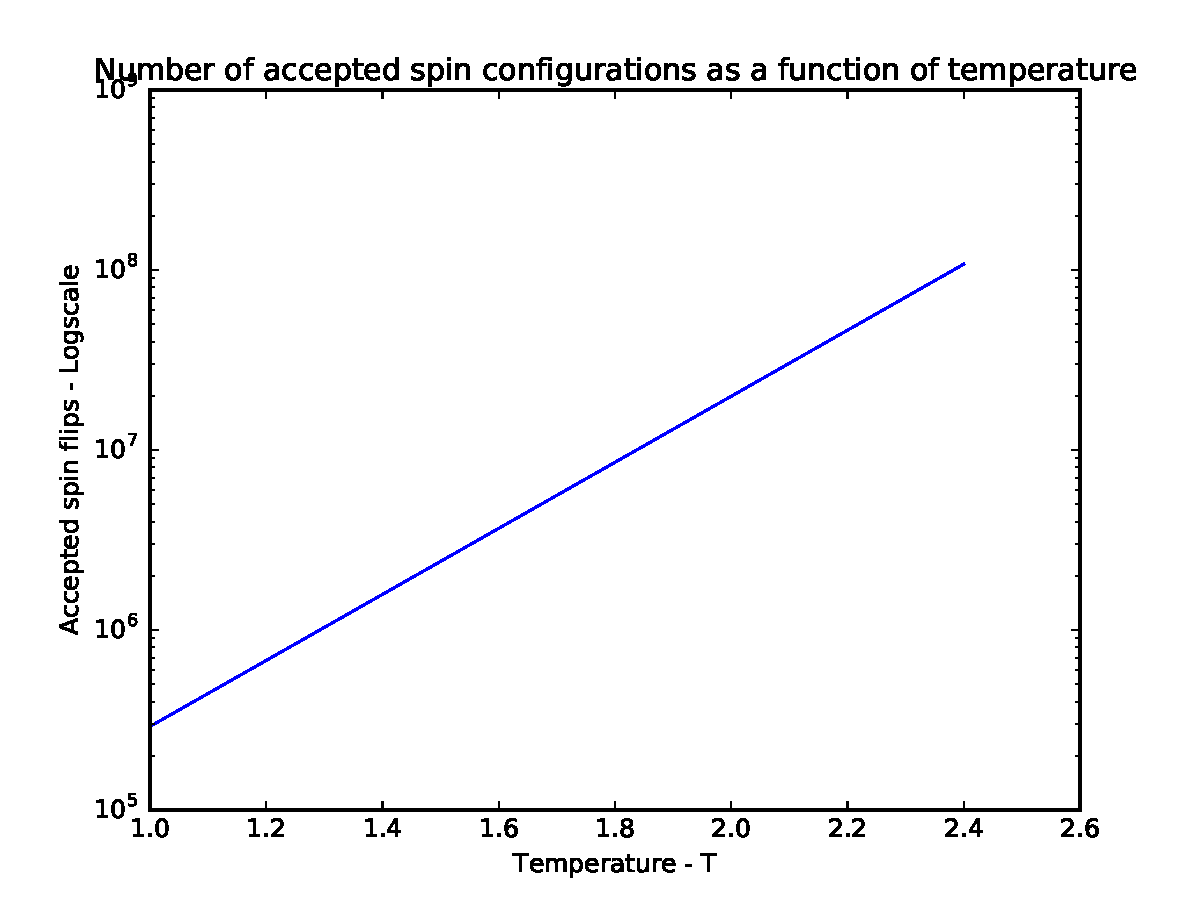
\includegraphics[width=\linewidth]{Plots/Accepted_configs_wrt_temp.pdf}
\caption{Number of accepted configurations for the two different temperatures. Logarithmic y-axis. Shows only two temperature points, so the increase may not be linear.}
\label{fig:Accepted_configs_wrt_temp}
\end{figure}

\begin{figure}[H]
\centering
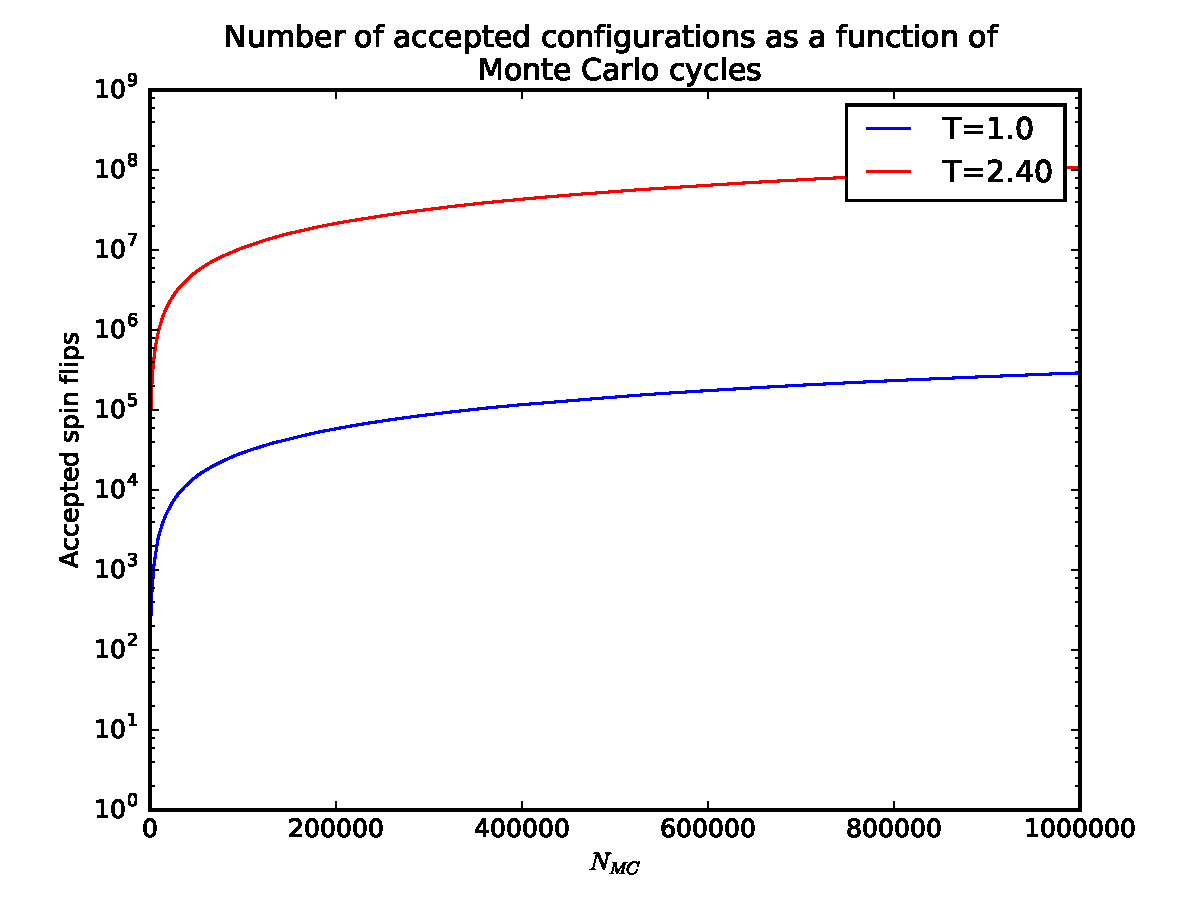
\includegraphics[width=\linewidth]{Plots/Accepted_configurations_wrt_MC_cycles.pdf}
\caption{Number of accepted configuration changes over time. Logarithmic y-axis. We see that the number of accepted configurations increases as the temperature increases}
\label{fig:Accepted_configs_wrt_MC_cycles}
\end{figure}


\FloatBarrier
\subsection*{Phase transitions}

\FloatBarrier
\section{Conclusion} \label{section:conclusion}

\FloatBarrier

\section{Appendix}
\begin{figure}[hbtp]
\centering
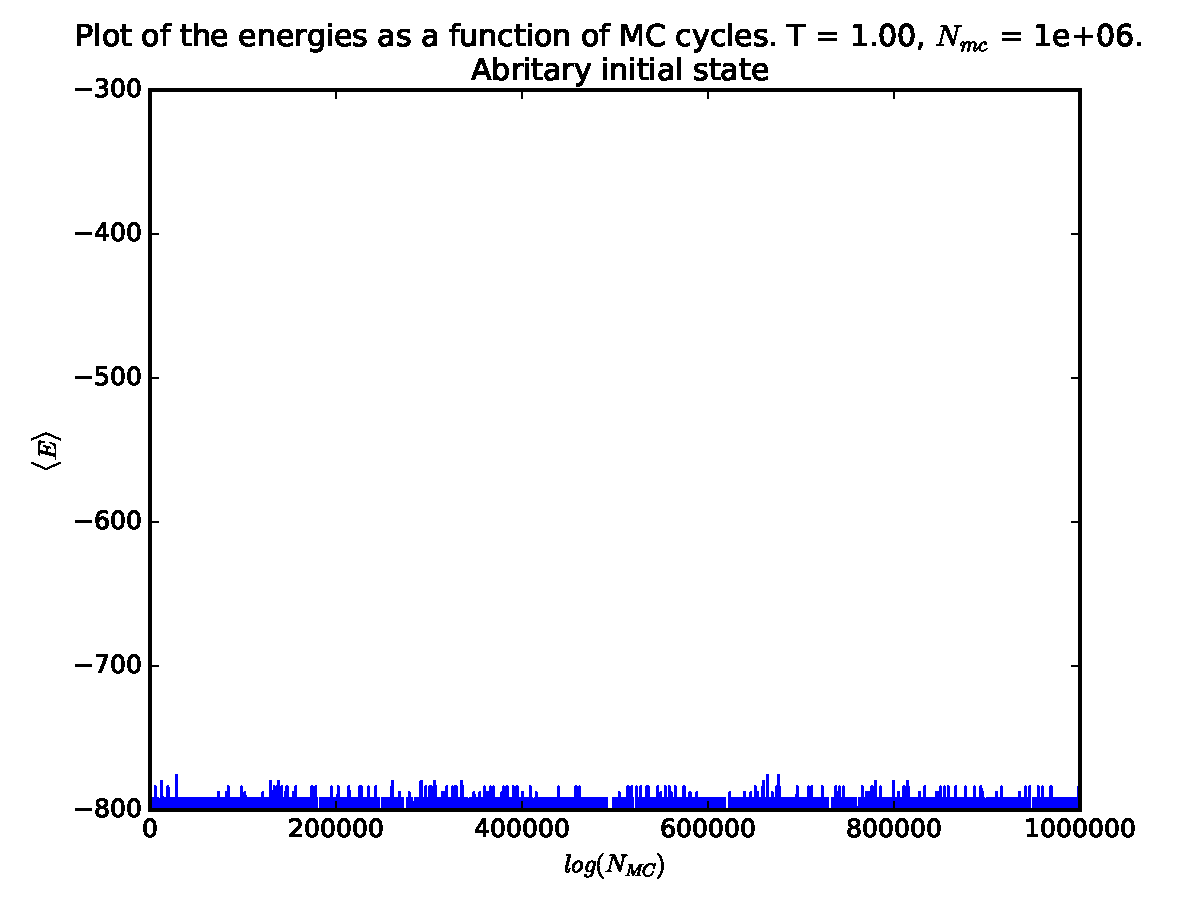
\includegraphics[width=\linewidth]{Plots/Energy_stability_T1.pdf}
\caption{Stability of the energy for T = 1.0.}
\end{figure}


\FloatBarrier
\begin{thebibliography}{1}
    \bibitem{cpyhsics} M. Hjorth-Jensen, \emph{Computational Physics}, 2015, 551 pages
\end{thebibliography}
\end{document}